\documentclass{article}

\author{Trever Hallock}
\title{Outline}

\usepackage[margin=0.5in]{geometry}
\usepackage{graphicx}

\begin{document}

\section{Introduction}

This paper will discuss constrained Derivative Free Optimization (DFO) with potentially narrow feasible regions.
Narrow constraints introduce numerical instability and make it hard to to form approximates for a function.
We have experimented with several strategies for handling hidden constraints.
The focus is on model-based trust region algorithms for local search within constrained derivative free optimization that maintain feasibility.



\section{}
We wish to solve problems of the form

\[ \begin{array}{ccl} \min & f(x) \\
\mbox{subject to} & c_i(x) \le 0 & i \in \mathcal{I} \\
& c_i(x) = 0 & i \in \mathcal{E}
\end{array}
\]

The feasible region is the set $\{x \in R \| c_i(x) = 0, i \in \mathcal{I} \wedge c_i(x) \le 0, \forall i \in \mathcal{E} \}$.


This problem becomes derivative free when derivative information about either $f$ or some $c_i$ is not available.
Depending on the nature of each of the functions, this can give rise to different type of problems.
We will assume that no derivative information is known of any function $f$ or $c_i$.
We will also make the assumption that no function can be evaluated outside of the feasible region $c_i(x) \le 0 \forall i \in \mathcal{I} \wedge c_i(x) = 0 i \in \mathcal{E}$.

Hidden constraints.


\section{Previous}
The classical algorithm handling when there are no constraints.


Define trust region subproblem.
Explain how to use model functions.
Update policy of the trust region radius.


\subsection{}
For convex problems, this fits within the gerneral framework presented in Global convergence of trust-region algorithms for convex constrained minimization without derivatives by P.D. Conejo.


\section{}
In order to handle constraints, we need to construct model functions of the constraints as well.
There are some issues with how to define this if we use different order model functions for the constraints as for the objective.
For now we will assume that we can evaluate the constraints exactly.

Our goal is to find an algorithm that will work when no derivative information is known.
However, in order to develop the algorithm, we begin with the assumption that the constraints are well known, and we can calculate the feasible region.

This does require feasible starting iterate.


\section{Algorithms}


\section{naive}
One simple approach to handling hidden constraints is to simply avoid letting points fall outside the feasible region.
Within this model, we maintain the same policies for updating the trust region radius.
However, within the LU factorization algorithm to select new points, we add to the trust region subproblem that the new points must also lie within the current model of the trust region.

This can happen when the feasible region intersect the trust region is small compared to the trust region.
As the number of dimensions grows, this can become worse.

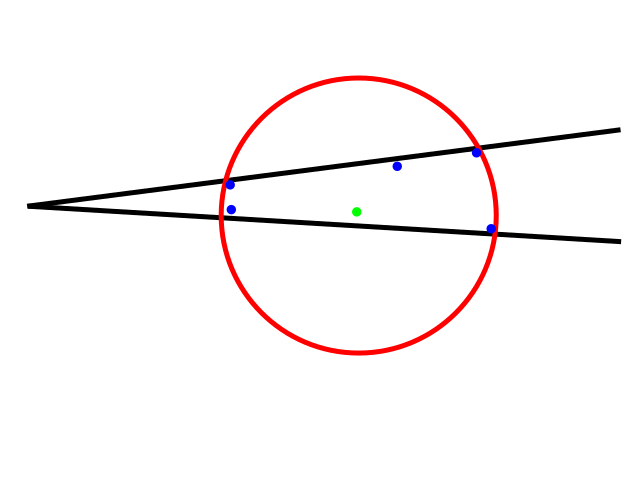
\includegraphics[scale=0.2]{bad_lambda.png}

\section{Bumping $\xi$}


Within the classical algorithm, we used $\xi$ as a lower bound of the pivot values of the Vandermode matrix.
When requiring points to live within the trust region intersect the feasible region, it can happen that even after replacing a point, we still have not satisfied this bound.
One way to handle this is to simply allow $\xi$ to decrease until a threshold is reached.
(The threshold is for maintaining a fixed lambda.)


    
\section{Ellipse}


We decided to keep the trust region entirely within the feasible region because of the high lambda when only requiring the points to lie in the feasible region.
In order to deal with the numerical problems from having a circular trust region, we can map the feasible region back to a circle.
More specifically, we define an ellipse $\{x \in R \| x^T (Q - c) x \le 1 \}$.
We then map this back to the origin with the affine transformation $T : R \to R$ $T(x) = L(x-c)$ where $L = cholesky(Q)^{-1}$.
This will allow us to construct a lambda poised set within narrow trust regions.


In order to do define the ellipse well, there are a number of problems to be solved.
One of the important decisions to be made is where the center of the ellipse is.
Also, we need to determine how to include the current iterate within the trust region.
This can be done by either expanding the radius of the ellipse, or by including the original point as a constraint for the ellipse problem.
If we do not include the current iterate, we may arbitrarly? decrease the function value.
Insert images here.

In order to include the original point as a constraint, we require that
$$
\bar{x}^T Q \bar{x} \le 1.
$$
Because this problem is stated in terms of the inverse, the problem has a constraint including the inverse of decision variables.

The alternative is to scale $Q$ by a constant to that this statement becomes true.
To do this we introduce a scaling factor $s$ of

$$ s = \max \{1, \frac 1 {2} (x^{current} - x^{center})^T Q (x^{current} - x^{center})^T \}$$

and let the ellipse be:
$$\{x | 1 - \frac 1 {2s} (x - x^{center})^T Q (x - x^{center}) \ge 0\} $$


The are some concerns we have to consider while defining the ellipse.
One major concern is that we can accidently define the ellise in a way that forces the trust region away from the desired drection.
Also, unless we include points outside the ellipse, we cannot find a second order solution because the ellipse can only be tangent to the constraint.
We also want consecutive ellipse to share volume, in order to avoid evaluating as many points as possible.
(So far, we have been re-evaluating the set of trial points each iteration.)
Finally, we have the problem of computing the ellipse once given a suitable definition.
Within this paper, we first solve the problem of finding the maximal ellipse given the center, and then perform a simple search over different centers of the ellipse.

\subsection{Finding the maximal ellipse given the center}




We are given a polyhedron $P$ defined by an $m \times n$ matrix $A$,
\[
P = \{ x \; | \;  Ax \le b \},
\]
and we wish to find the largest ellipse $E \subset P$ centered at a point $x^{\star}$ within this polyhedron.

We can shift the polyhedron by letting $\bar{b} = b - Ax^{\star}$ and letting $x \to x - x^{\star}$ so that the polyhedron becomes
\[
P = \{ x \; | \;  Ax \le \bar{b} \}
\]
The ellipse can then be centered at zero, and defined by a positive semi-definite matrix $Q \succeq 0$:
\[
E = \{ d \; | \; \frac 1 2 d^T Q d \le 1 \}.
\]
where $Q = Q^T$.
We can define the auxiliary function 
\[
f(x) = \frac 1 2 x^T Q x
\]
so that this becomes
\[
E = \{ d \; | \; f(d) \le 1 \}.
\]


At the locations where the ellipse intersects the polyhedra with minimum value of $f$, the gradients of $f$ must be orthogonal to the faces.
Each face is defined by at least one $A_i x \le \bar{b}_i$ where $A_i$ is the $i$th row of $A$ for $1\le i \le m$.
This implies that if $d^{(i)}$ is such a point, then
\[
\nabla f(d^{(i)}) = \lambda_i A_i \quad \forall 1\le i\le m
\]
for some $\lambda_i$.
This means
\[
Q d^{(i)} = \lambda_i A_i \quad \forall 1\le i\le m
\]
\[
d^{(i)} = \lambda_i Q^{-1}A_i \quad \forall 1\le i\le m
\]
We also know that 
\[
A_i^T d^{(i)} = \bar{b} \quad \forall 1\le i\le m
\]
\[
A_i^T \lambda_i Q^{-1}A_i = \bar{b} \quad \forall 1\le i\le m
\]
\[
\lambda_i = \frac {\bar{b}}{A_i^T  Q^{-1}A_i} \quad \forall 1\le i\le m
\]
so that 
\[
d^{(i)} = \lambda_i Q^{-1}A_i \forall 1\le i\le m
\]
\[
d^{(i)} = \frac {\bar{b}}{A_i^T  Q^{-1}A_i}  Q^{-1}A_i \quad \forall 1\le i\le m.
\]

Finally, we need that for each $i$, $f(d^{(i)}) \le 1$:
\[
\frac 1 2 (d^{(i)})^{T} Q d^{(i)} \le 1
\]
\[
\frac 1 2 (\frac {\bar{b}}{A_i^T  Q^{-1}A_i}  Q^{-1}A_i)^{T} Q \frac {\bar{b}}{A_i^T  Q^{-1}A_i}  Q^{-1}A_i \le 1
\]
\[
\frac 1 2 \frac {1}{A_i^T  Q^{-1}A_i}  \bar{b}^T A_i^T Q^{-1} Q \frac {\bar{b}}{A_i^T  Q^{-1}A_i}  Q^{-1}A_i \le 1
\]
\[
\frac 1 2 \frac {1}{A_i^T  Q^{-1}A_i}  \bar{b}^T \frac {\bar{b}}{A_i^T  Q^{-1}A_i}  A_i^T Q^{-1}A_i \le 1
\]
\[
\frac 1 2 \bar{b}^T \frac {\bar{b}}{A_i^T  Q^{-1}A_i} \le 1
\]
\[
\frac 1 2 \bar{b}^T \bar{b}\le A_i^T  Q^{-1}A_i
\]
\[
A_i^T  Q^{-1}A_i \ge \frac 1 2 \bar{b}^T \bar{b}
\]

Thus, the maximal ellipse is defined by

\[
\sup_{Q \succeq 0} \det(Q^{-1})
\]
\[
s.t. \quad A_i^T Q^{-1} A_i \ge \frac 1 2 \bar{b}^T\bar{b}
\]


The problem difficulty includes a maximization of a determinant


\subsection{Stationary center}
The simplest approach is to not change the center of the ellipse, but instead keep it at the current center.
In the example below, we begin with a trust region that must be very small to lie within the feasible region, and note that if we even keep the same center, we are still able to search towards the vertex of the feasible region.
After solving the trust region subproblem in the first image, the iterate is near a constraint within the next iteration.
However, the ellipse elongates along an axis parallel to this constraint.

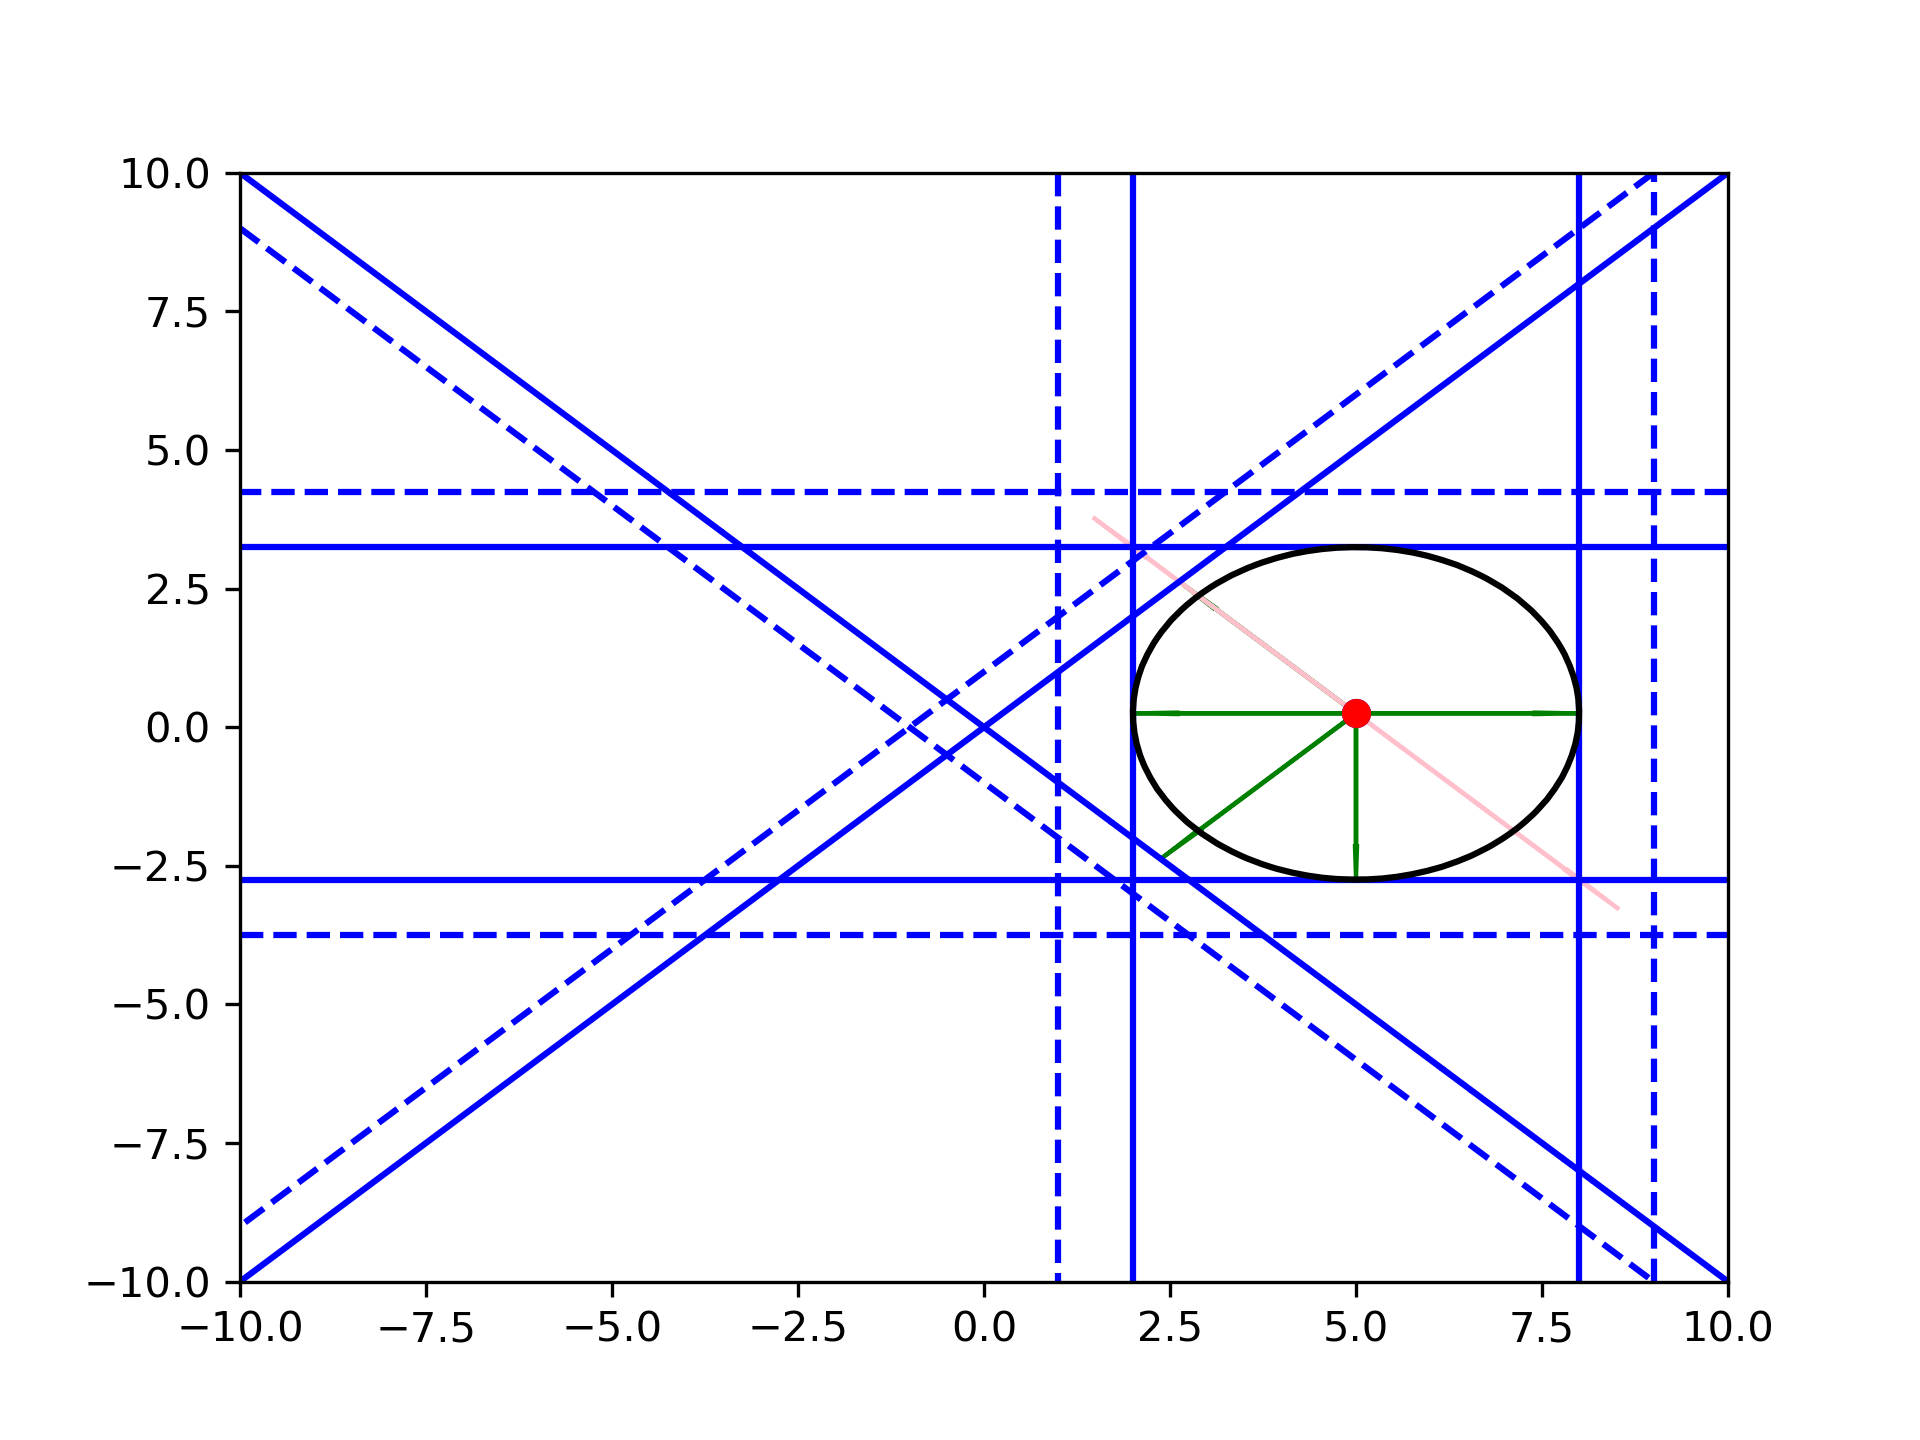
\includegraphics[scale=0.2]{advantage_of_ellipse_1.png}
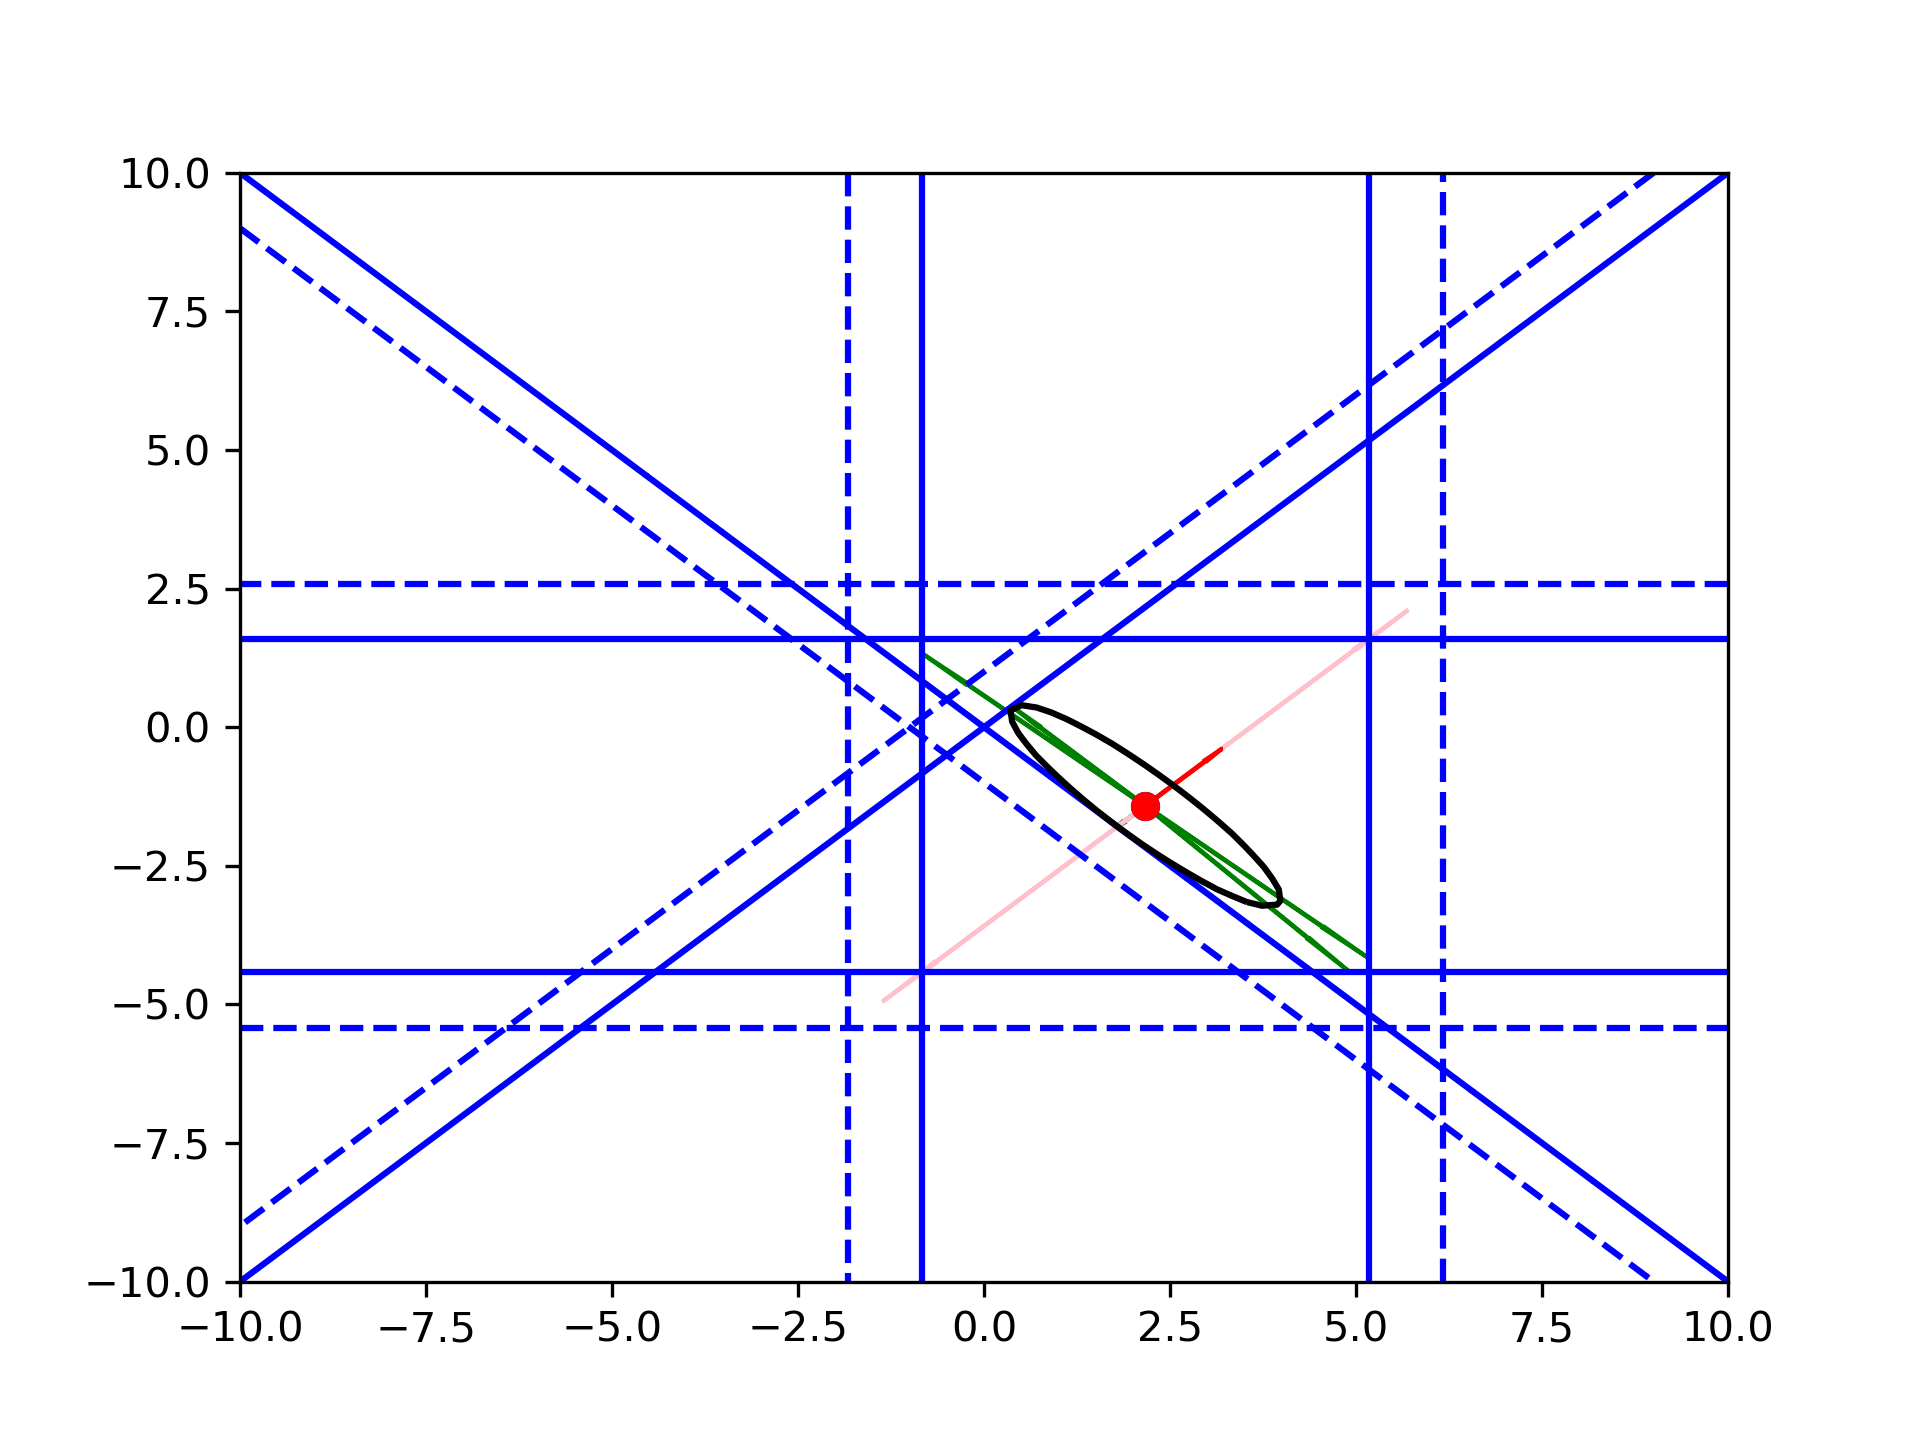
\includegraphics[scale=0.2]{advantage_of_ellipse_2.png}



\subsection{Search everything}
Another simple approach is to define the ellipse as to maximize the area within the ellipse.
Assuming that that we are modelling the constraints with linear functions, this means that we define the ellipse by minimizing the determinant of $Q$.
This has the advantage that it captures much of the feasible region.


However, one problem with this search is that it can force the trust region away from the desired direction.

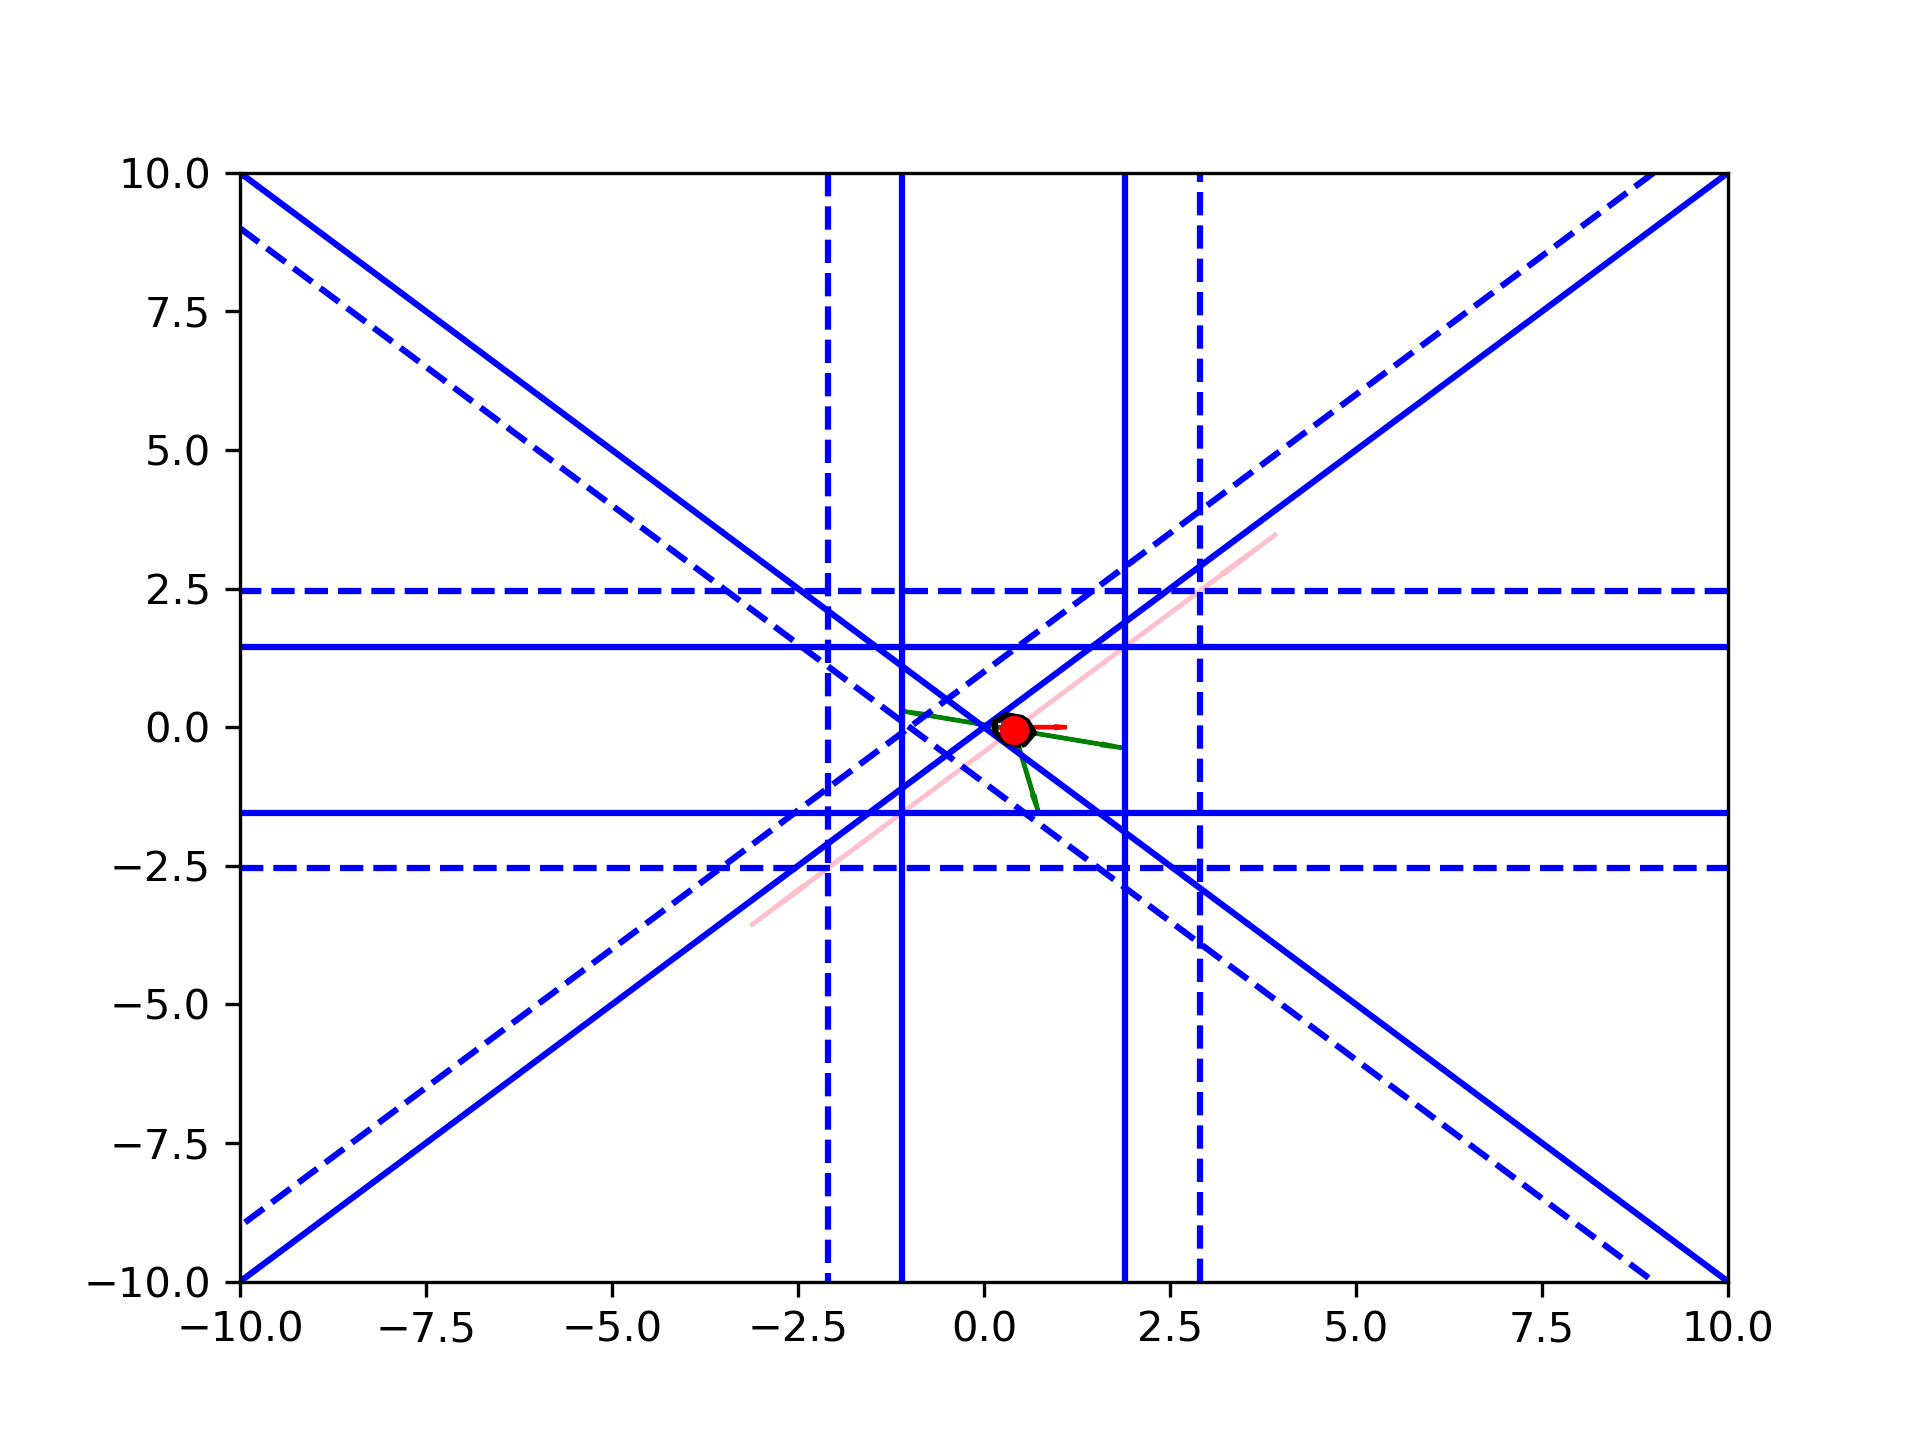
\includegraphics[scale=0.2]{everything_runs_1.png}
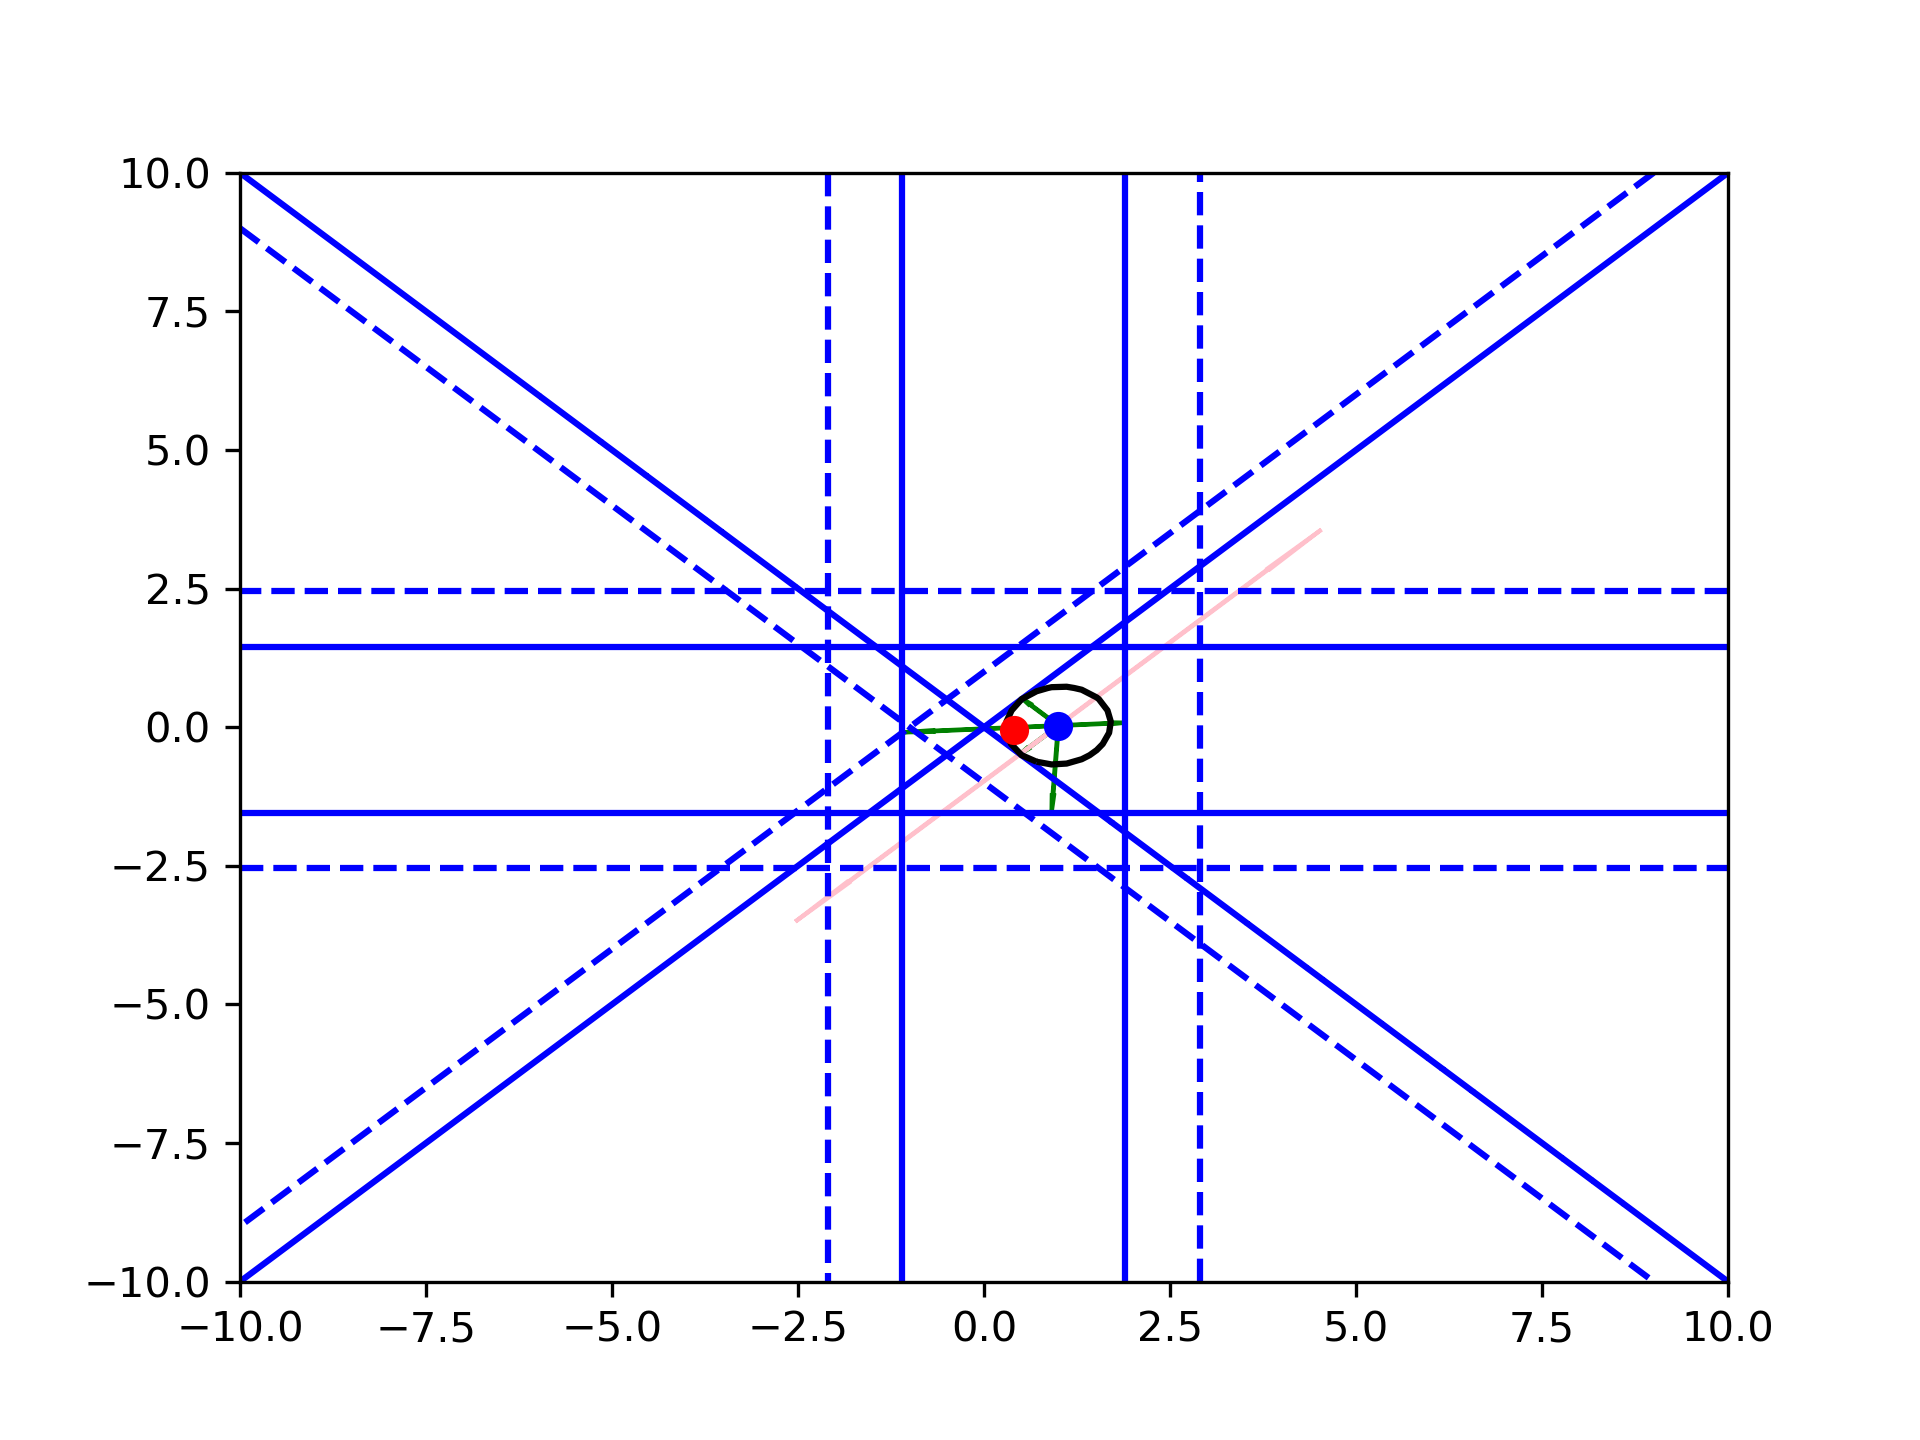
\includegraphics[scale=0.2]{everything_runs_2.png}


One attempt to fix this problem is by limiting the search direction for the center of the ellipse.

\subsection{Line searches}
Although the minimum of problem $P$ can appear anywhere within the trust region, there are some reasons for expecting it to be at a ``vertex."
If it lies on the interiorer, there is little need for using constrained approaches once near the solution.

The ellipse with maximum volume, however, tends to lead away from vertices because there is more space away from vertices.
One way of trying to leave the direction towards a vertex within the trust region, while still allowing to incease the ellipse volume is by limiting the search for the new center to lie on line segments starting at the current iterate.

For example, our first attempt was to simply search a line directed away from the closest constraint.
This has obvious problems though, as we should avoid letting the new center get closer to another constraint:

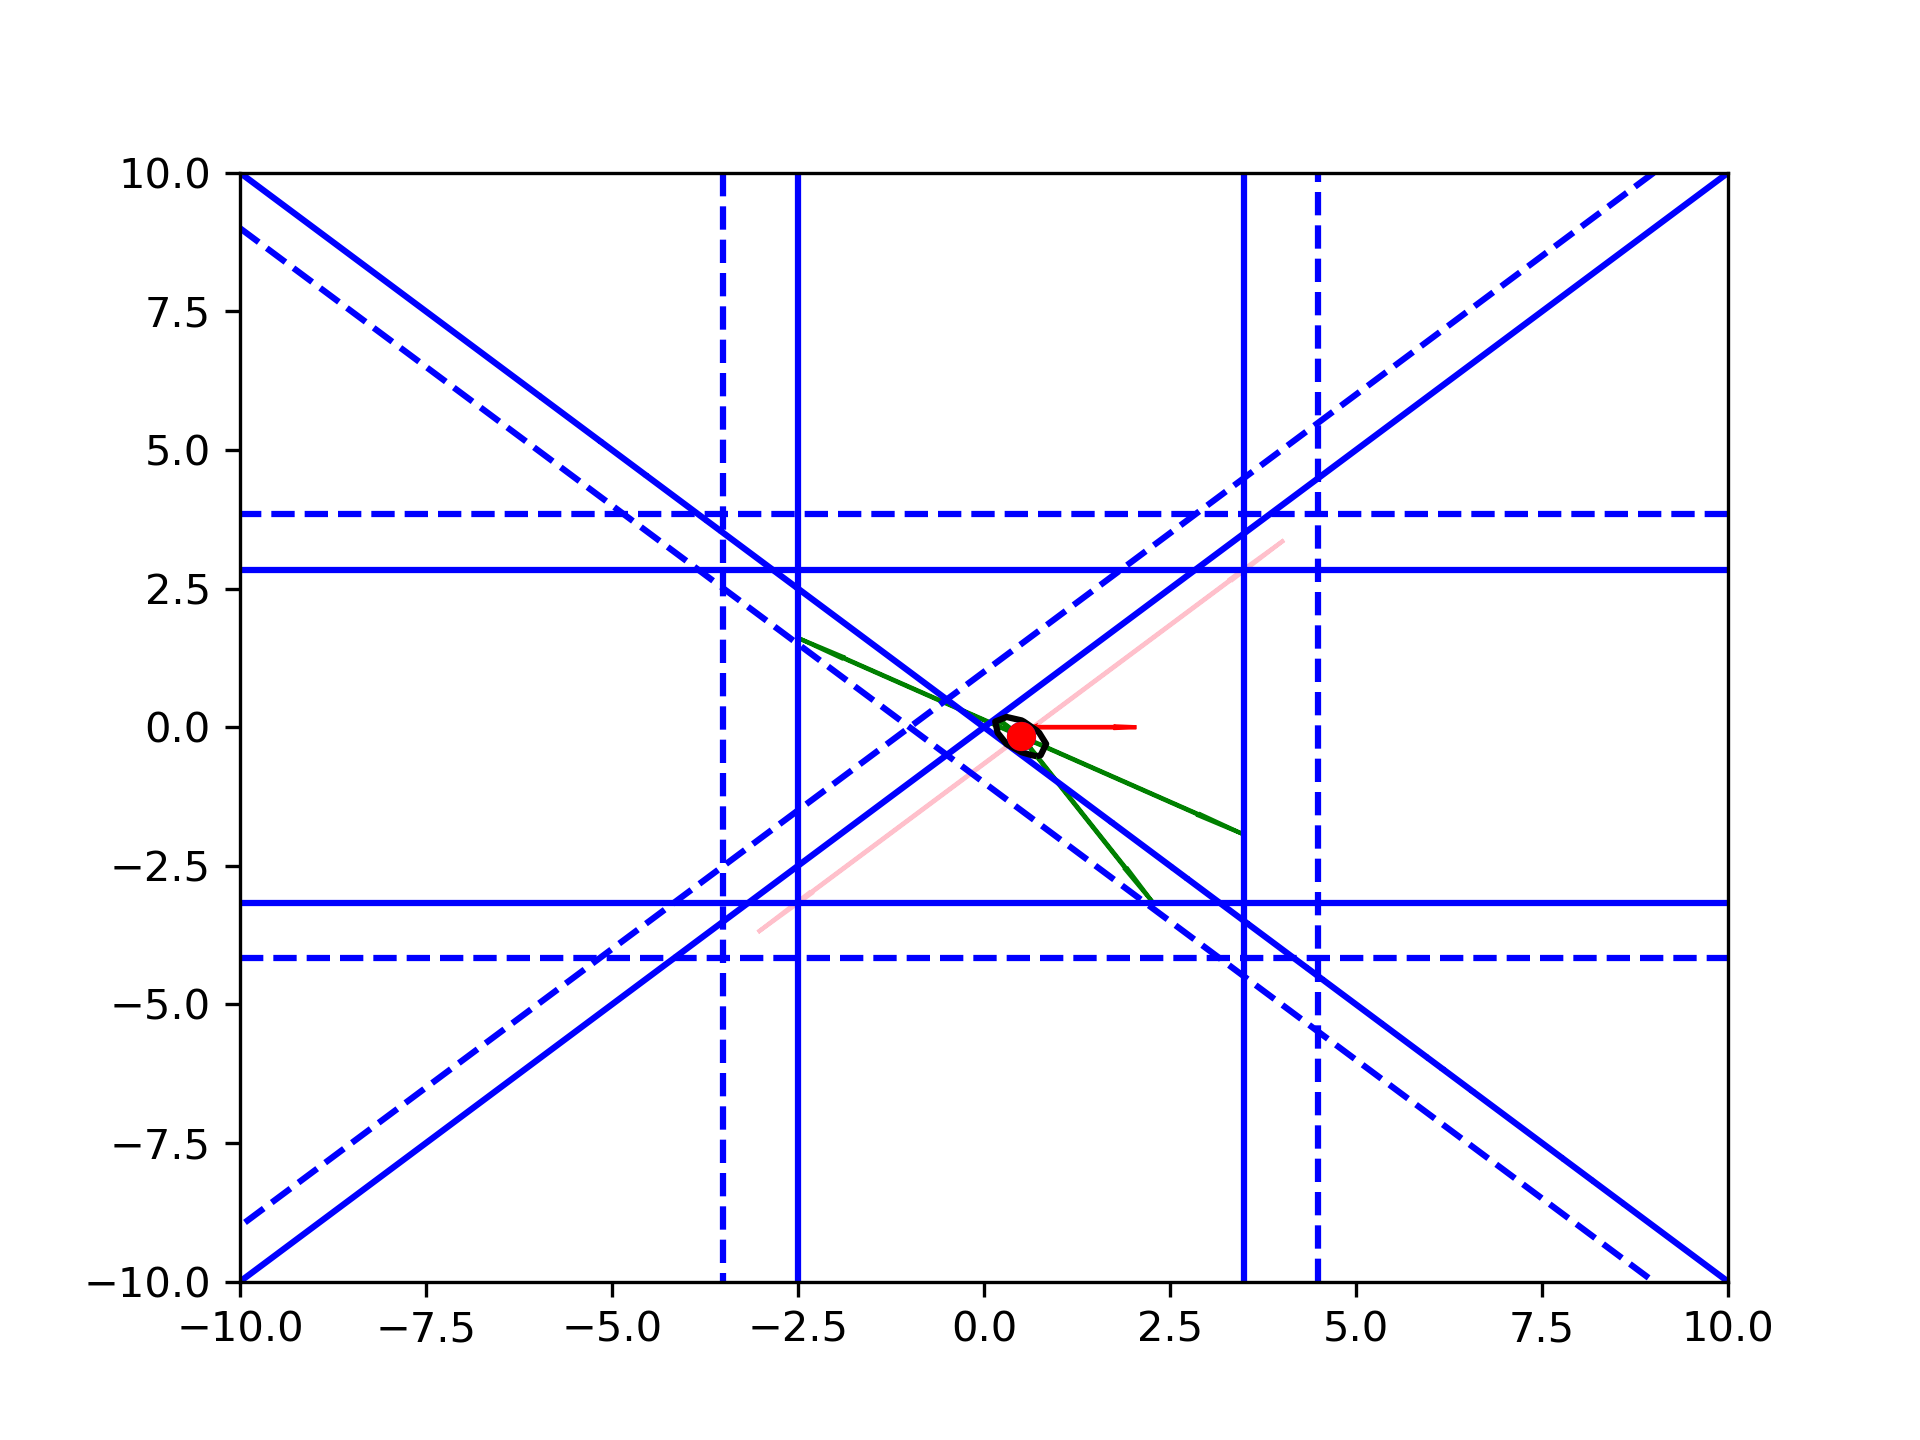
\includegraphics[scale=0.2]{line_1.png}
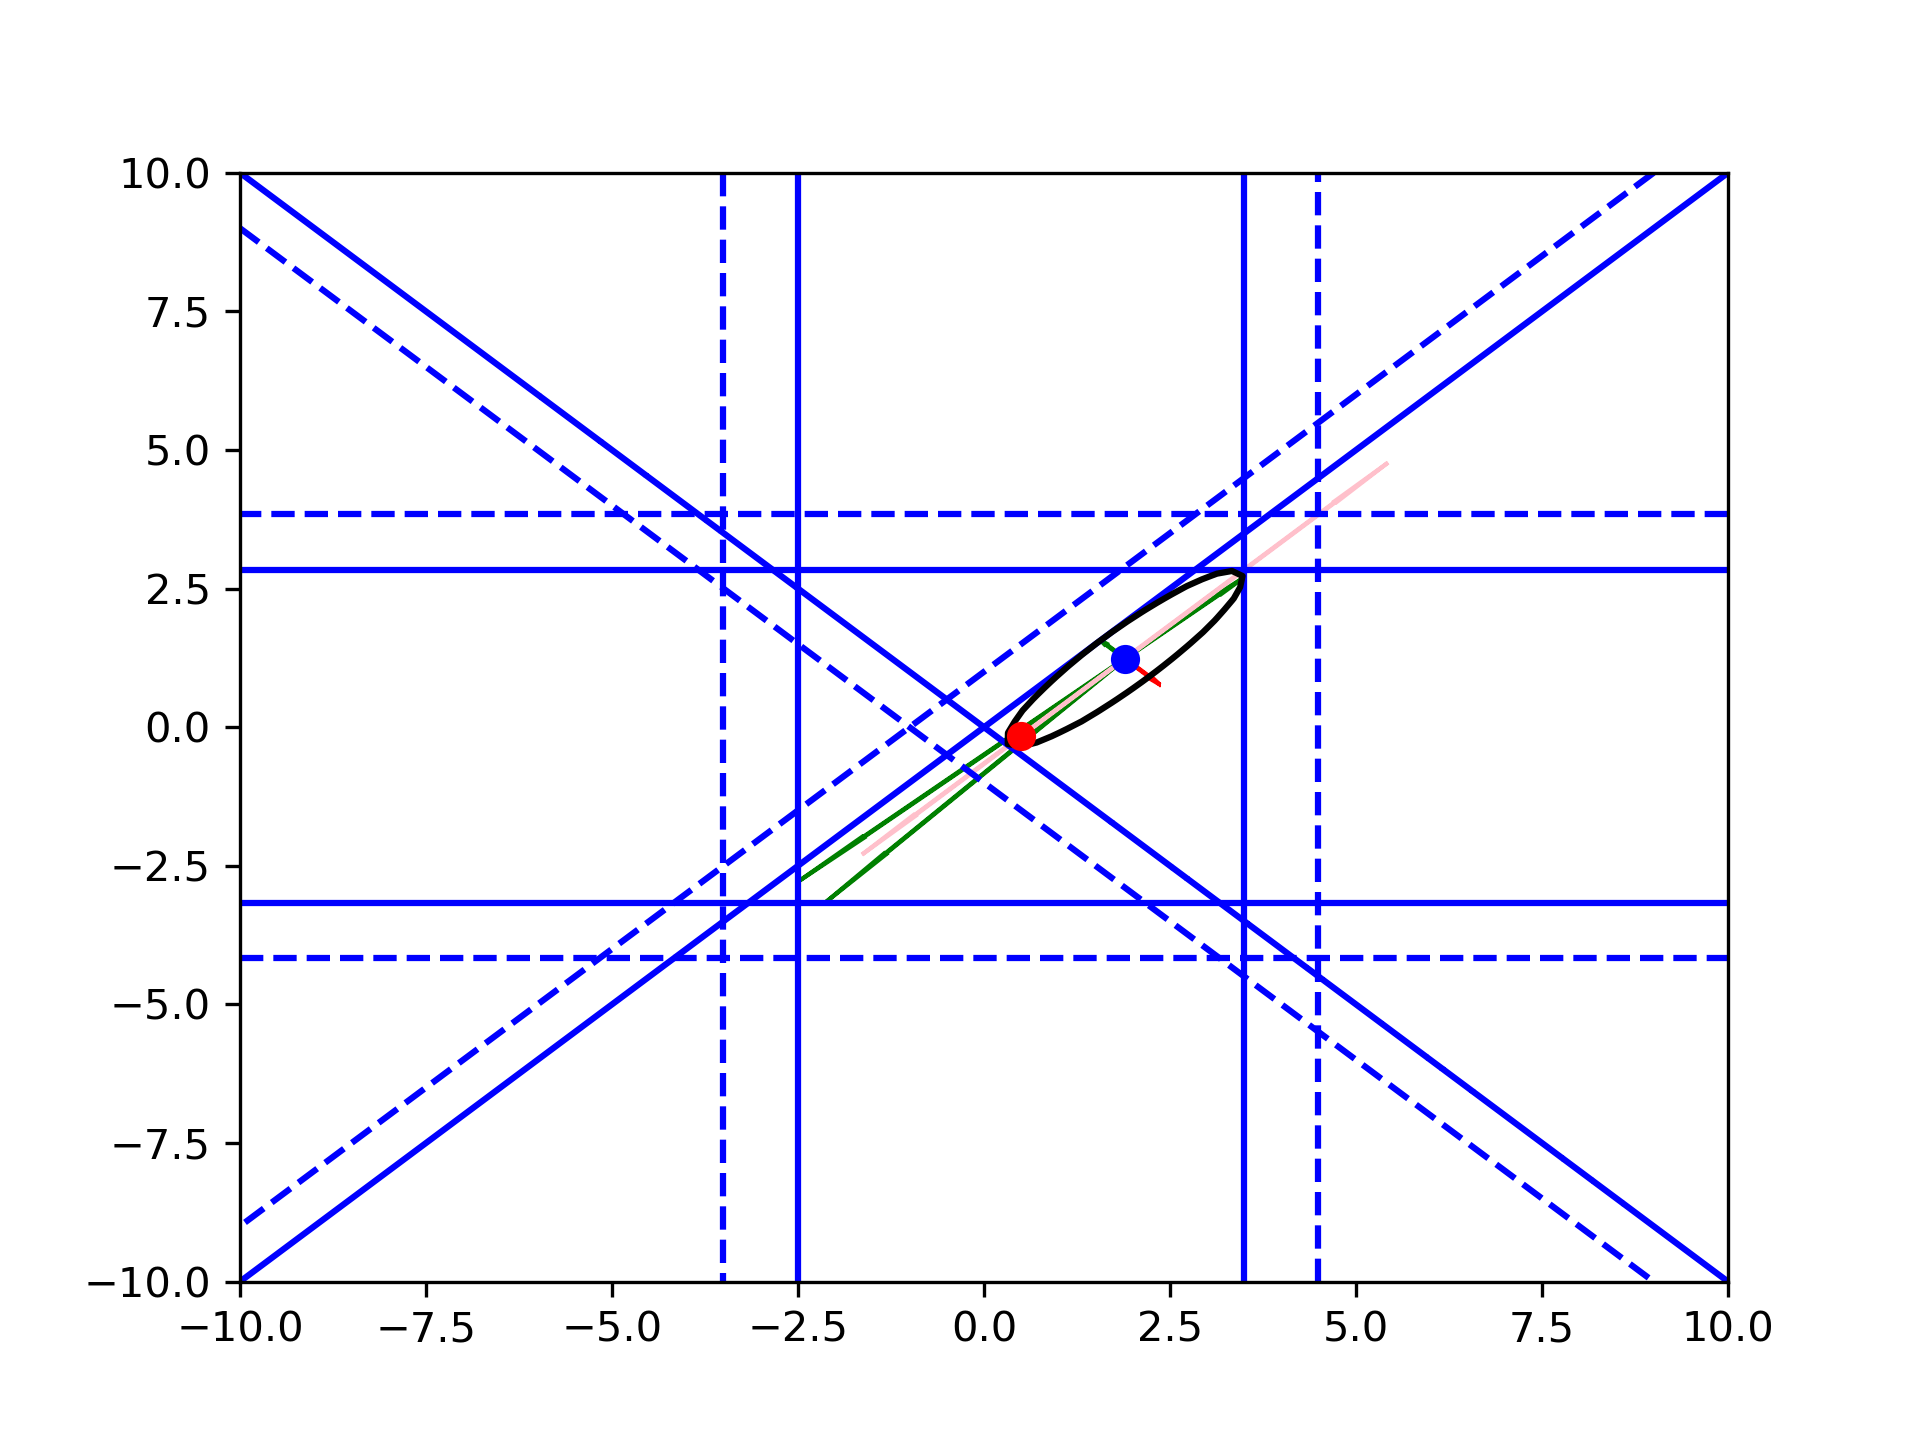
\includegraphics[scale=0.2]{line_2.png}


To fix this, we break the line into segments based on the nearest constraint.
We find the center that maximizes the volume of the ellipse after restricting it to lie on a ray perpendicular to the nearest constraint.
Nearest here means means the constraint with the smallest distance from the iterate to the projection of that iterate onto the constraint.
If there are two constraints that are both closer than all others, then we follow a ray whose points are equidistant from both of these constraints.

We search along this away from the current iterate until we reach a point that has the same distance to another constraint as the nearest to the iterate.
We could then in general continue to follow line segments by always travelling away from the nearest constraints.
However, after we include enough constraints, we will eventually once again head away from a vertex.

This means that we can define the a class of searches that each use a different number of line segments to search.
In this paper, we consider one and two line segments.

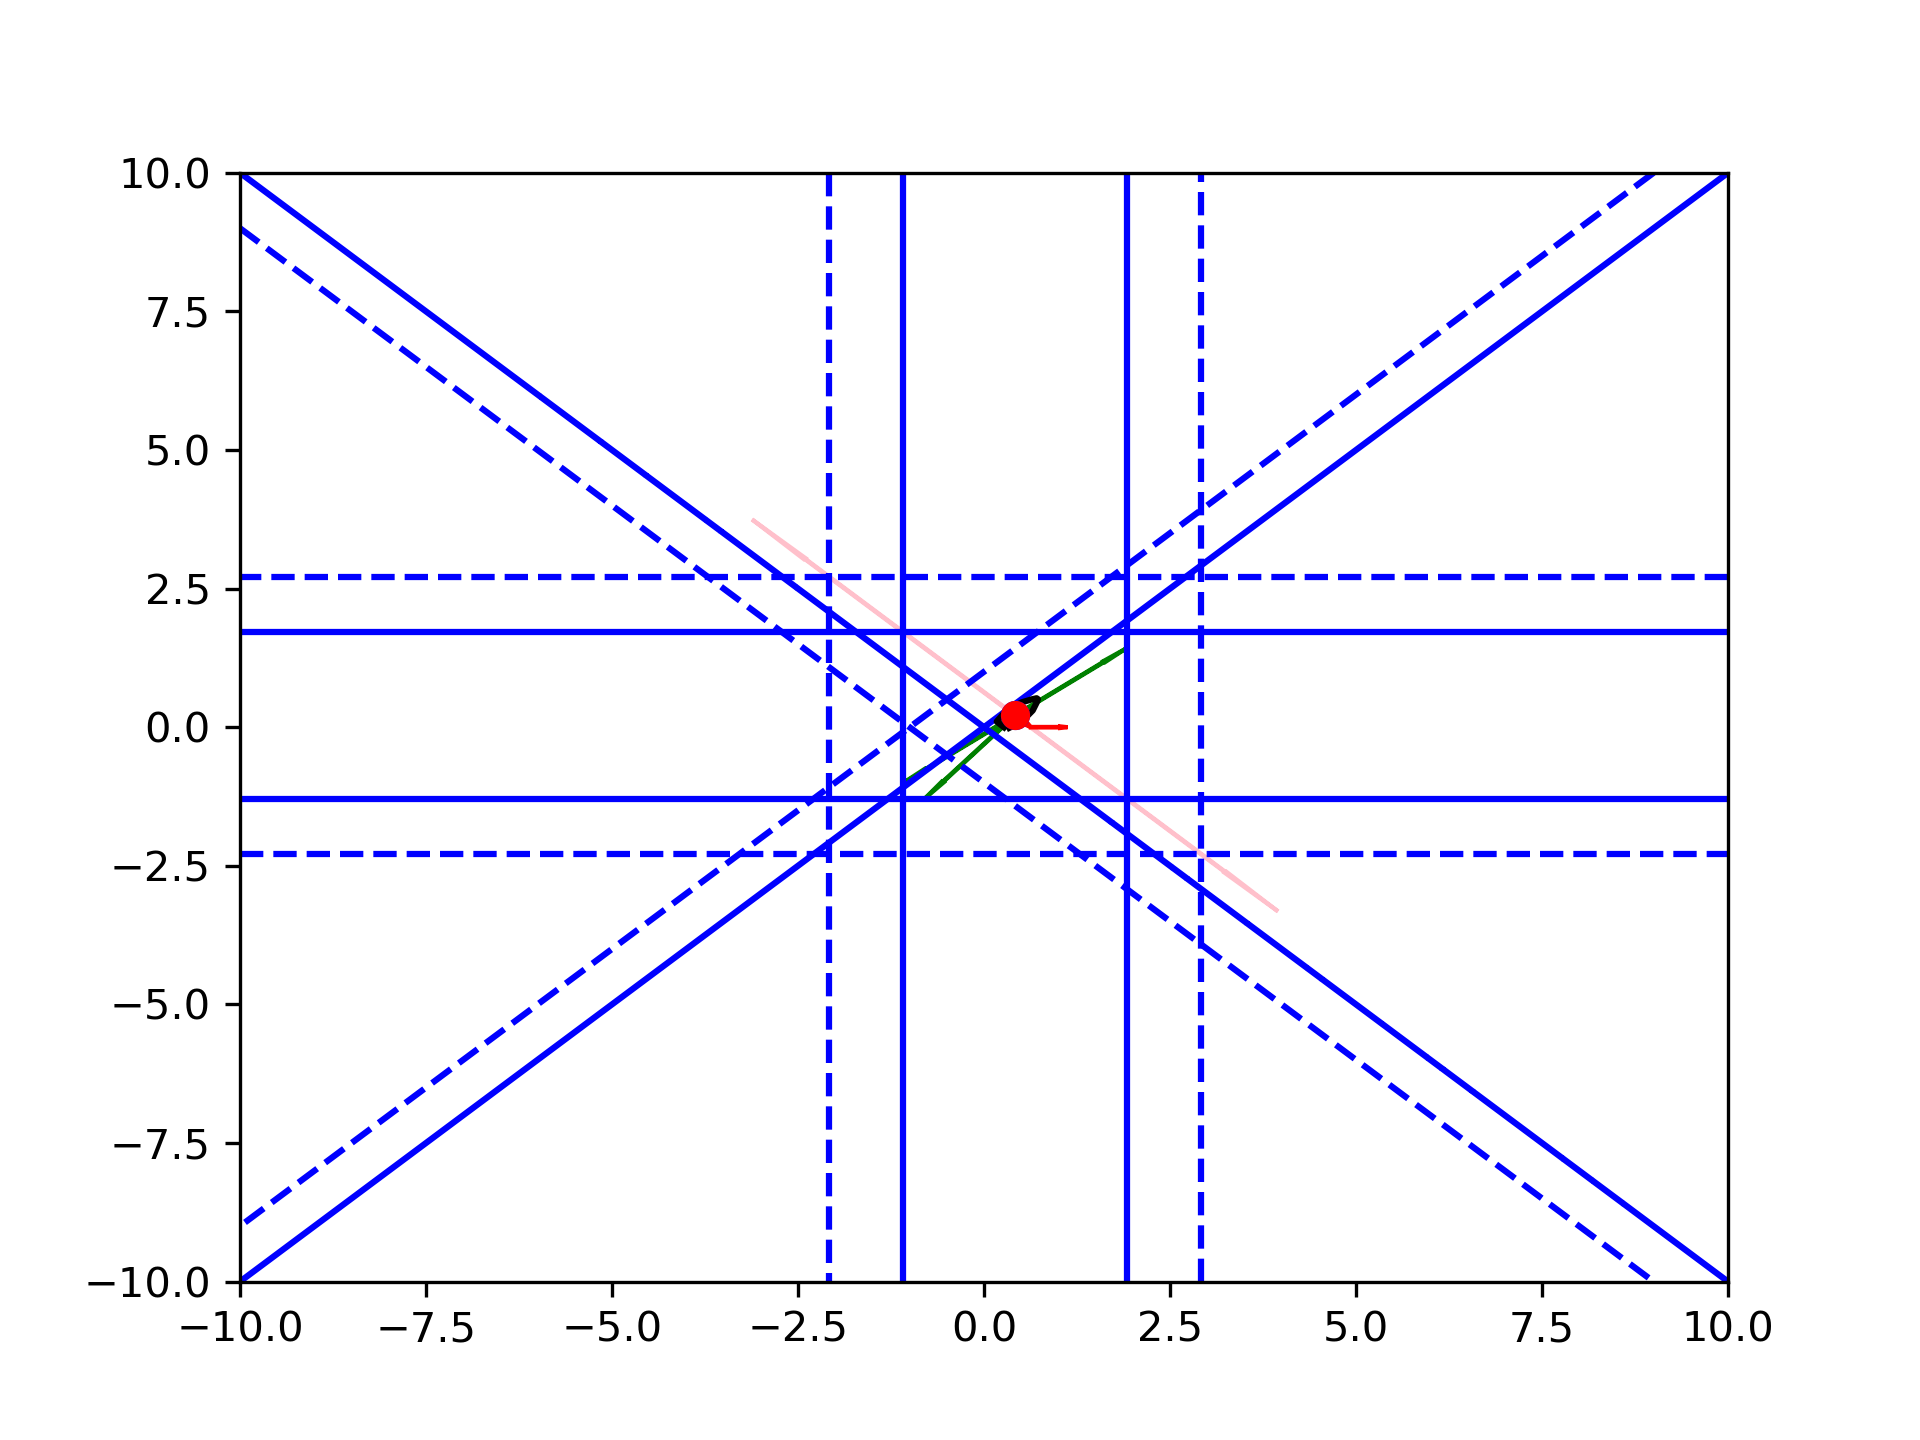
\includegraphics[scale=0.2]{run_away_1.png}
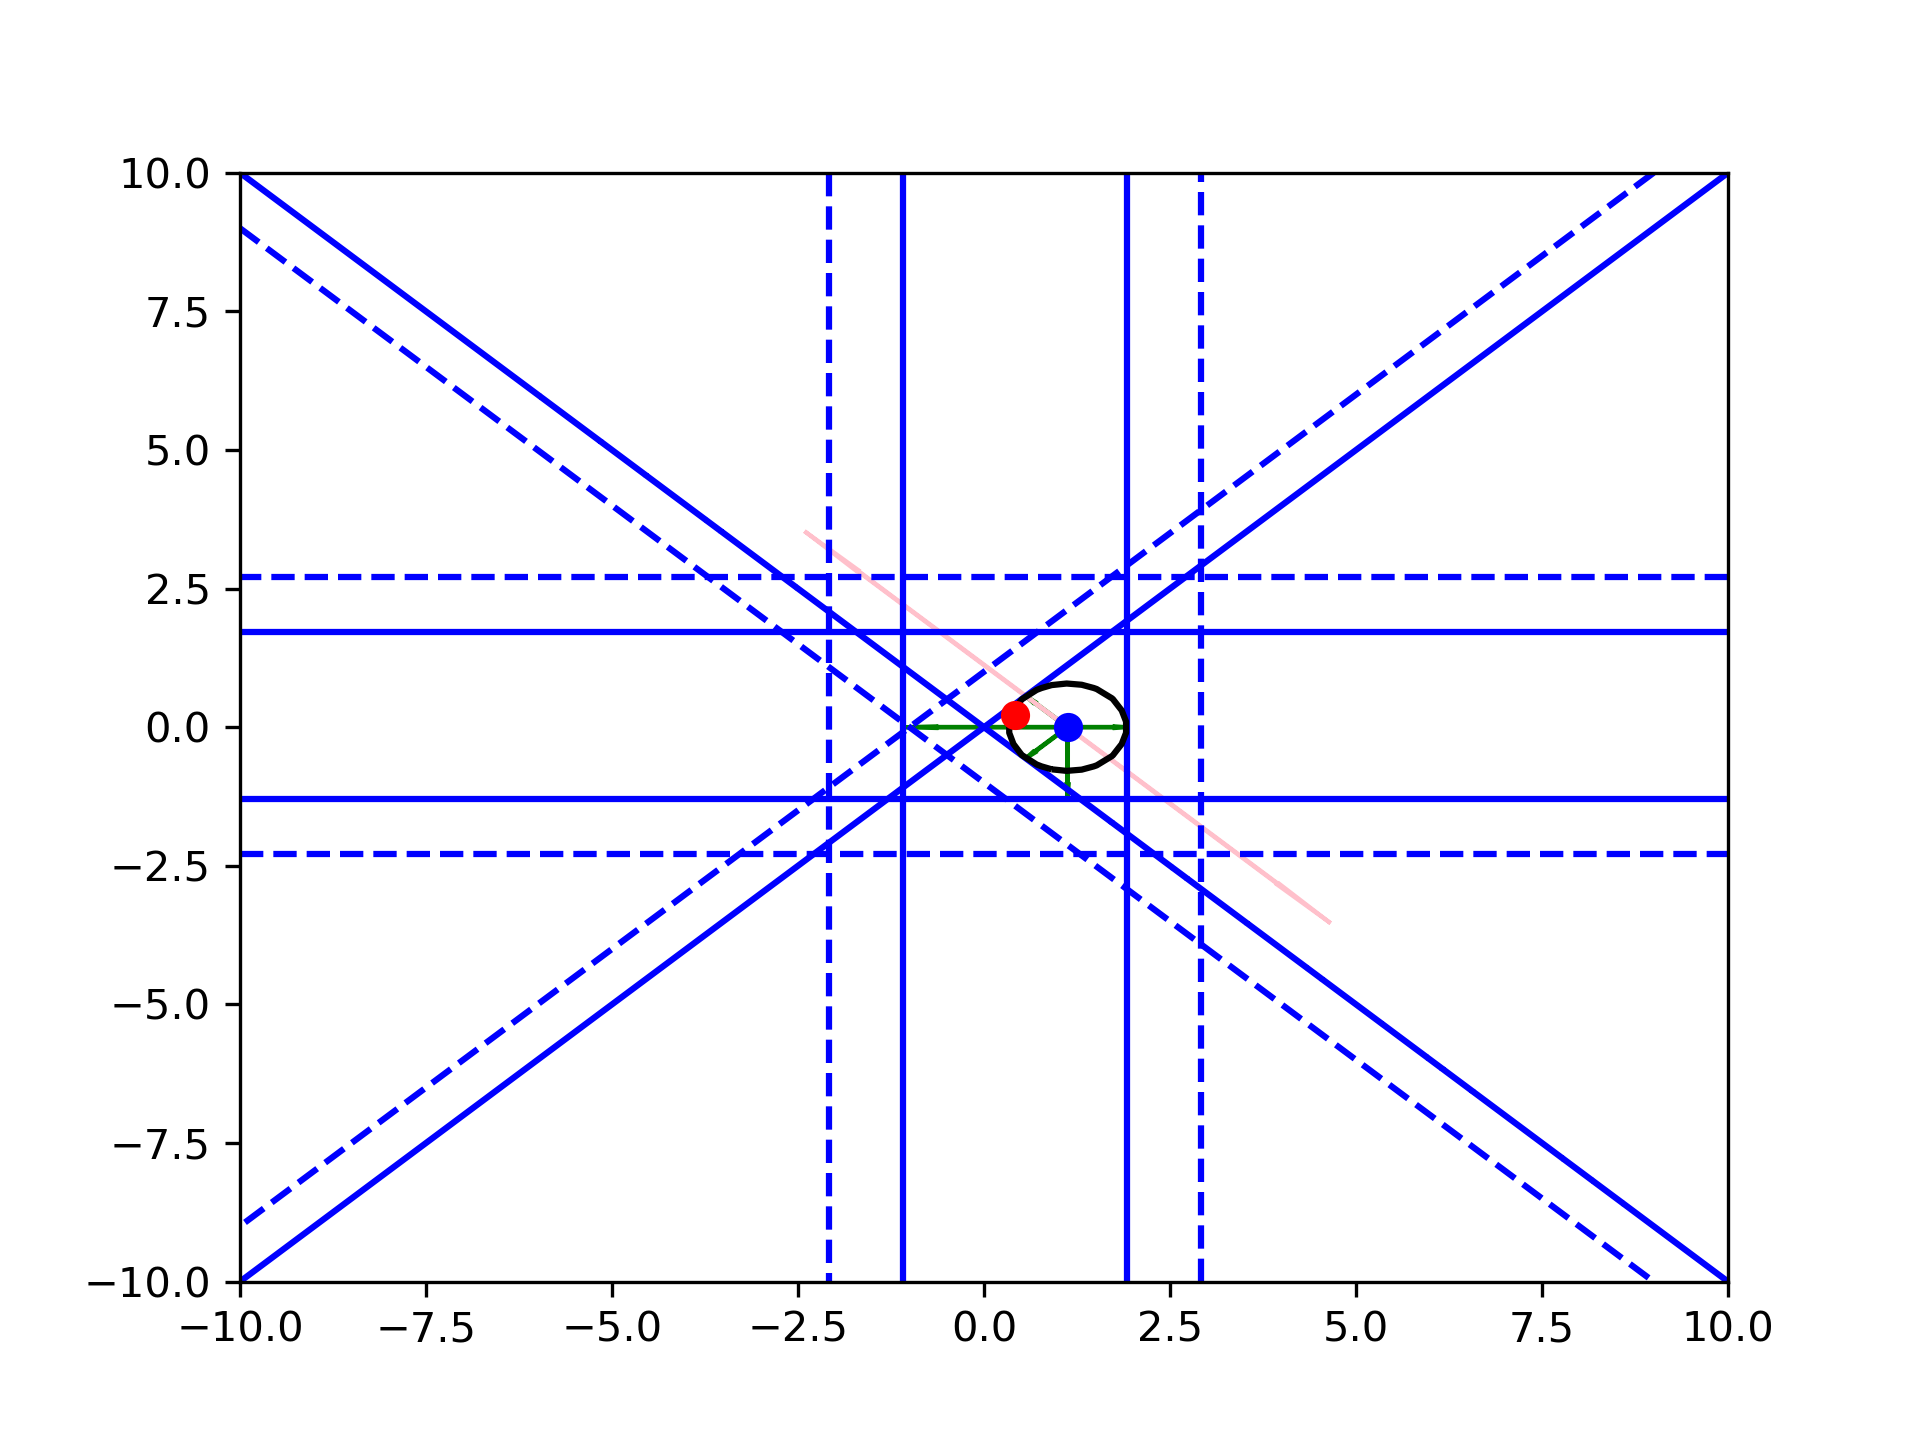
\includegraphics[scale=0.2]{run_away_2.png}

\section{Results}

the example problem I have been working with
    linear constraints
%\min \alpha sin(x) + \beta (minor * x + (y - self.amplitude * x sin(freq * x)) ^ 2 
%
%		return 0.9 * (x[0]) + 0.1 * (self.minorSpeed * x[0] + (x[1] - self.amplitude * x[0] * sin(self.freq * x[0])) ** 2)





\begin{center}
\begin{tabular}{ c c c }
 Algorithm & Iterations & Evaluations \\ 
 Search everything (include the original) & 24 & 169 \\  
 Search everything & 19 & 106    \\
 One line segment & 21 & 86 \\
 Two line segments & 23 & 115 \\
\end{tabular}
\end{center}

\end{document}



